\documentclass{article}

\usepackage{graphicx}
\usepackage{tikz}
\usepackage{tikzsymbols}
\usetikzlibrary{calc,patterns,shapes.geometric}
\pagestyle{empty}
\usepackage[margin=0pt]{geometry}
\geometry{papersize={14in,12in}}

\def\centerarc[#1](#2)(#3:#4:#5){\draw[#1] ($(#2)+({#5*cos(#3)},{#5*sin(#3)})$) arc (#3:#4:#5);}

\begin{document}
	\begin{figure}
		\centering
		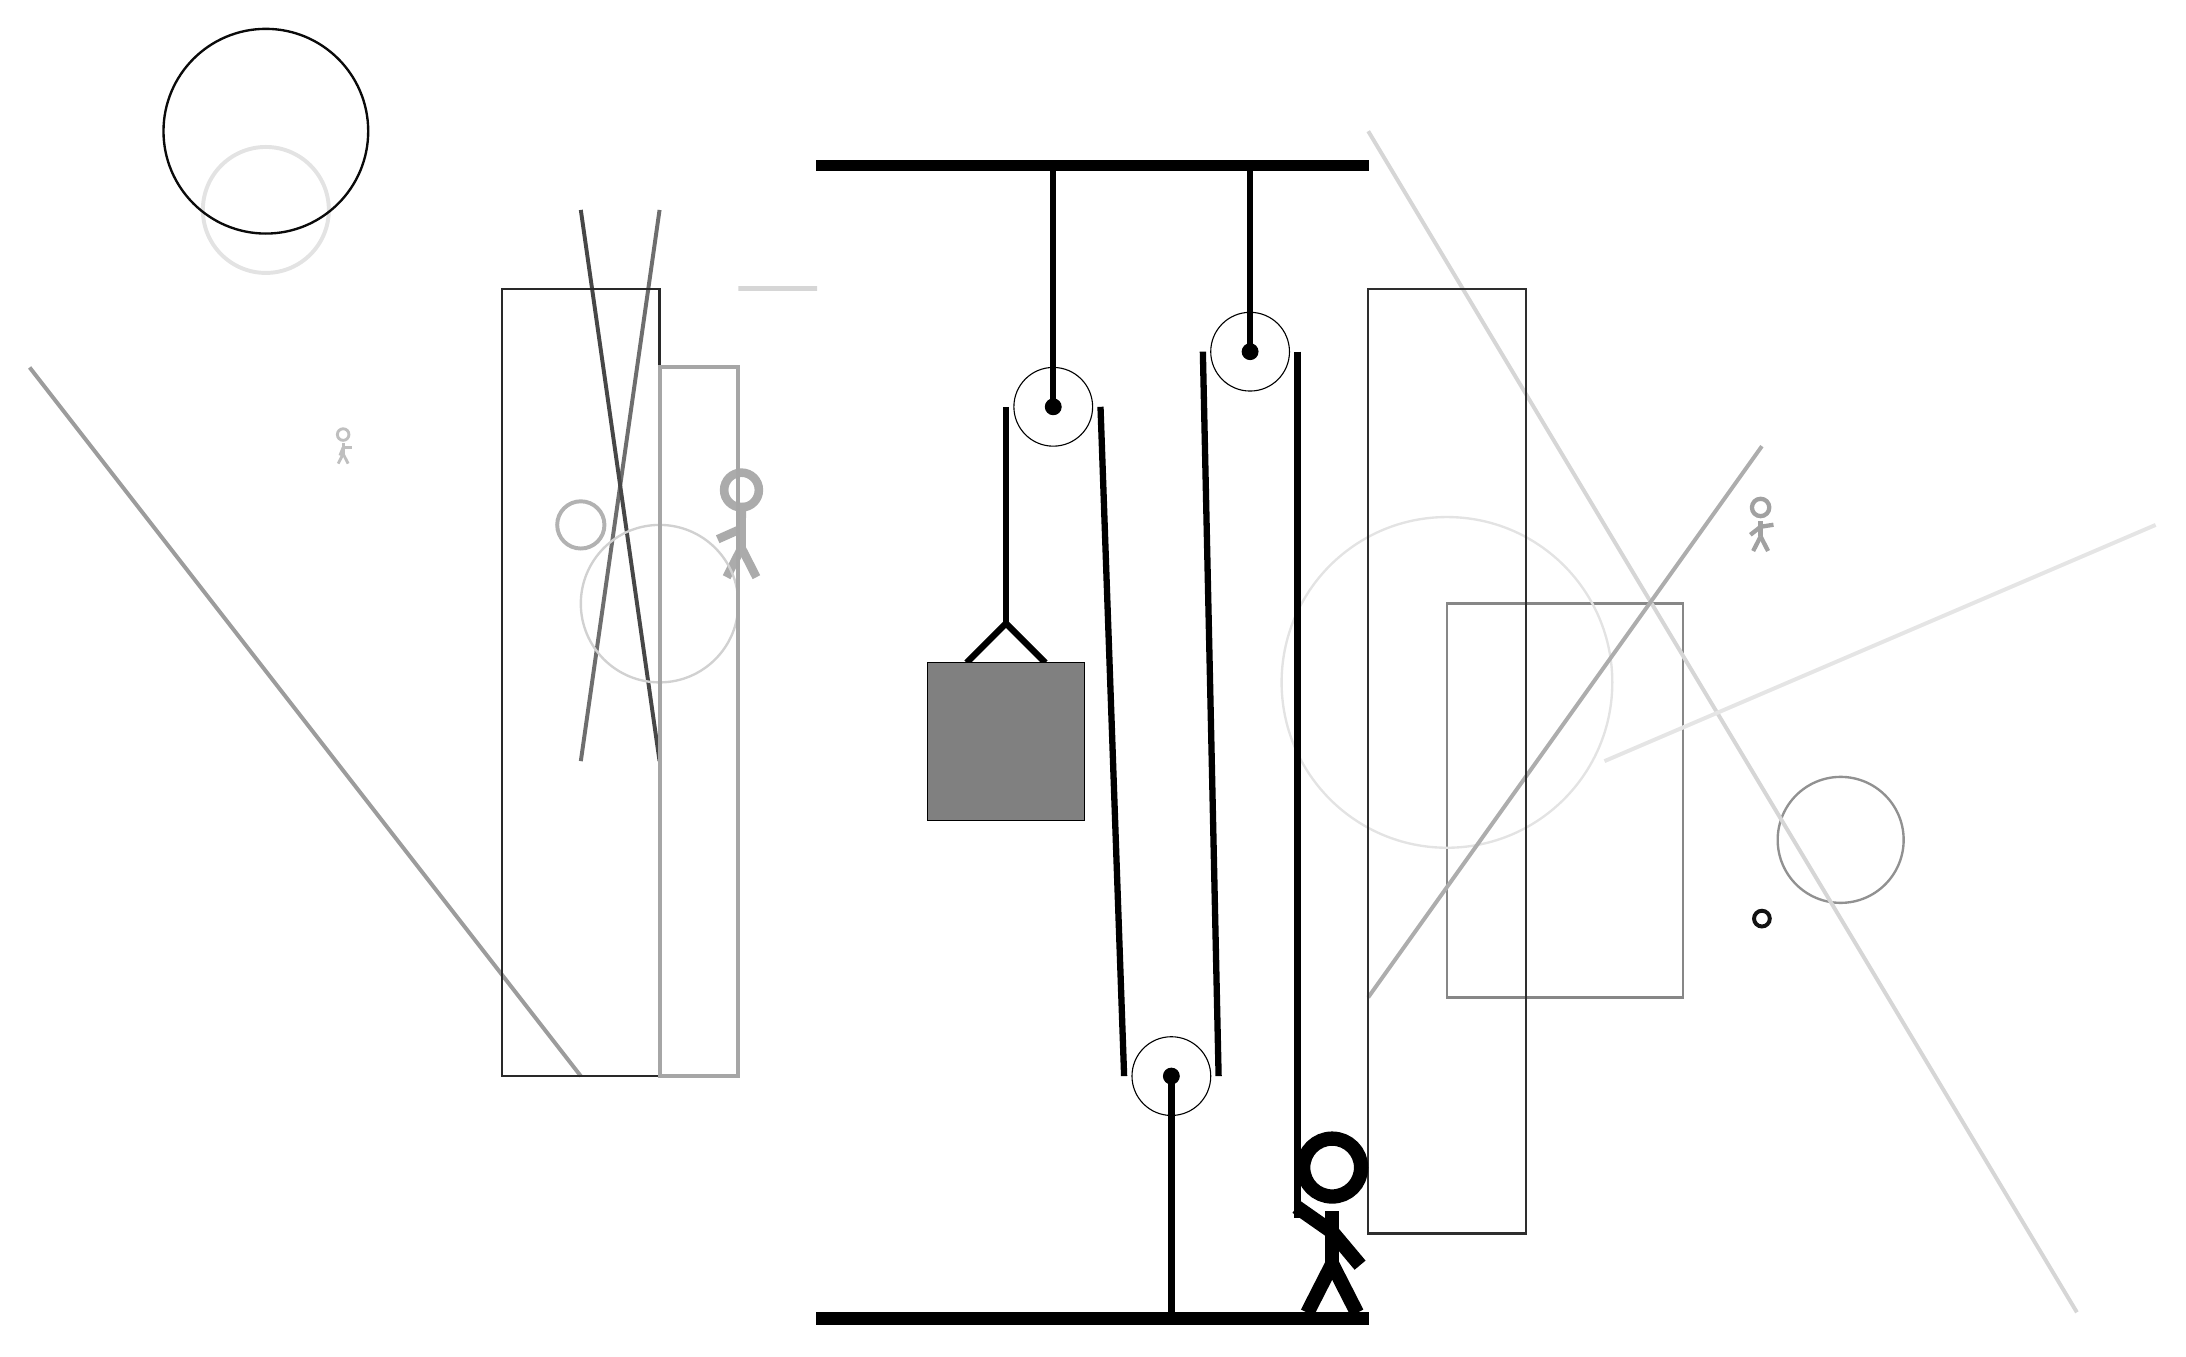
\begin{tikzpicture}
			%%%%% START %%%%%
			
			\draw[fill=black] (-2, 11.5) rectangle (5, 11.625);
			
			\draw (1, 8.5) circle (0.5);
			\draw[fill=black] (1, 8.5) circle (0.1);
			\draw[line width=0.8mm]  (1, 11.5) -- (1, 8.5);
			
			\draw[line width=0.5mm, color=black!57](-4, 11) -- (-5, 4);
			
			\draw [line width=0.5mm, color=black!11](-9, 11) circle (0.8);
			\draw[line width=0.5mm, color=black!72](-5, 11) -- (-4, 4);
			\draw [line width=0.3mm, color=black!96](-9, 12) circle (1.3);
			\draw [line width=0.5mm, color=black!30](-5, 7) circle (0.3);
			
			\draw[line width=0.6mm, color=black!16] (-2, 10) rectangle (-3, 10);
			\draw[line width=0.5mm, color=black!39](-5, 0) -- (-12, 9);
			\node[line width=0.7mm, color=black!25] at (-8, 8) {\Strichmaxerl[2][68][0]};
			\draw [line width=0.3mm, color=black!43](11, 3) circle (0.8);
			\draw [line width=0.5mm, color=black!93](10, 2) circle (0.1);
			
			\draw[line width=0.3mm, color=black!47] (6, 6) rectangle (9, 1);
			\draw[line width=0.5mm, color=black!16](5, 12) -- (14, -3);
			\draw [line width=0.3mm, color=black!11](6, 5) circle (2.1);
			
			\draw[line width=0.5mm, color=black!32](10, 8) -- (5, 1);
			\node[line width=0.5mm, color=black!37] at (10, 7) {\Strichmaxerl[3][38][9]};
			\node[line width=0.2mm, color=black!33] at (-3, 7) {\Strichmaxerl[6][24][89]};
			
			\draw[line width=0.3mm, color=black!84] (-4, 0) rectangle (-6, 10);
			\draw[line width=0.5mm, color=black!10](8, 4) -- (15, 7);
			\draw[line width=0.3mm, color=black!82] (5, 10) rectangle (7, -2);
			
			\draw [line width=0.3mm, color=black!18](-4, 6) circle (1.0);
			\draw[line width=0.5mm, color=black!35] (-4, 9) rectangle (-3, 0);
			
			
			\draw[fill=white](2.5, 0.0) circle (0.5);
			\draw[fill=black] (2.5, 0.0) circle (0.1);
			\draw[line width=0.8mm]  (2.5, -3) -- (2.5, 0.0);
			
			\draw[fill=white](3.5, 9.2) circle (0.5);
			\draw[fill=black] (3.5, 9.2) circle (0.1);
			\draw[line width=0.8mm] (3.5, 11.5) -- (3.5, 9.2);
			
			\draw[line width=0.8mm] (-0.1, 5.25) -- (0.4, 5.75) -- (0.9, 5.25);
			\draw[fill=black!50] (-0.6, 5.25) rectangle (1.4, 3.25);
			
			\draw[line width=0.8mm] (0.4, 8.5) -- (0.4, 5.75);
			\centerarc[line width=0.8mm](1, 8.5)(0:180:0.6);
			\draw[line width=0.8mm](1.6, 8.5) -- (1.9, 0.0);
			\centerarc[line width=0.8mm](2.5, 0.0)(180:360:0.6);
			\draw[line width=0.8mm](3.1, 0.0) -- (2.9, 9.2);
			\centerarc[line width=0.8mm](3.5, 9.2)(0:180:0.6);
			\draw[line width=0.8mm](4.1, 9.2) -- (4.1, -1.8);
			
			\node at (4.5, -1.9) {\Strichmaxerl[10][-35][-50]};
			
			\draw[fill=black] (-2, -3) rectangle (5, -3.15);
			
			%%%%% END %%%%%
		\end{tikzpicture}
	\end{figure}	
\end{document}